\documentclass{beamer}
\usetheme{Warsaw}
\usepackage[brazilian]{babel}
\usepackage[utf8]{inputenc}
\usepackage{algorithm2e}

\AtBeginSection[]
{
	\begin{frame}<beamer>
		\frametitle{Agenda}
		\tableofcontents[currentsection,currentsubsection]
	\end{frame}
}


% Dados para o slide inicial da apresentação. %
\title{Estudo e Implementação de Ordenação por Reversão Com Sinal}
\author{Fernando Chirigati, Rafael Dahis, Rafael Lopes, Victor Bursztyn}
\institute[UFRJ]{
	Biologia Computacional
	
	Engenharia de Sistemas e Computação 
	
	Mestrado em Engenharia de Sistemas e Computação 
	
	Universidade Federal do Rio de Janeiro
	
	Professoras Celina e Marília
}
\date[Maio 2011]{30 de Maio de 2011}

% Fim dos dados para o slide inicial da apresentação. %

% Iniciando slides %
\begin{document}

% Slide inicial %
\begin{frame}[plain]
  \titlepage
\end{frame}

% Aqui começamos a apresentação %

\section{Introdução}

\begin{frame}
	\begin{itemize}
		\item Comparar genomas = descobrir a distância entre genes
 		\item Reversão = um tipo de operação de reorganização das bases de um gene
 		\item Ordenação por reversão = reordenar uma cadeia utilizando somente reversões
 	\end{itemize}

	\begin{figure}
		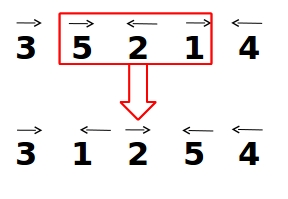
\includegraphics[scale=0.5]{./imagens/img_01.jpg}
	\end{figure}
\end{frame} 	
 	
\section{Implementação}
\subsection{Dados iniciais}

\begin{frame}
	\begin{itemize}
		\item Desenvolvimento em C
		\item Alocação dinâmica de memória
 		\item Limitação de Escopo: não consideramos tratamento de componentes ruins
 		\pause \item Mas devemos sempre fazer o teste!
 		\pause \item Algoritmo termina se encontrar alguma componente ruim
	\end{itemize}
\end{frame}

\subsection{O algoritmo}

\begin{frame}
	\begin{itemize}
		\item Desenvolvido por Hannenhalli e Pevzner em 1995.
		\item Baseado no Diagrama de Realidade e Desejo(DRD).
 		\item Complexidade alta.
	\end{itemize}
\end{frame}

\begin{frame}{Conceitos}
	\begin{itemize}
		\item Arestas divergentes $\to$ ao dar orientação em um ciclo, duas arestas de desejo que estão em sentidos opostos no DRD.
		\pause \item Arestas convergentes $\to$ caso as arestas de desejo estejam no mesmo sentido.
		\pause \item Ciclo bom $\to$ um ciclo que possui ao menos duas arestas divergentes.
		\pause \item Ciclo ruim $\to$ um ciclo que todas as arestas são convergentes.
		\pause \item Componente de um diagrama $\to$ todos os ciclos que se cruzam formam uma componenete.
		\pause \item Componente boa $\to$ possui ao menos um ciclo bom.
		\pause \item Componente ruim $\to$ todos os ciclos são ruins.
	\end{itemize}
\end{frame}

\begin{frame}
	\begin{block} {Algoritmo}
		\begin{algorithm}[H]
			\SetKwInOut{Entrada}{entrada}\SetKwInOut{saida}{Saida}
			\Entrada{Permutação $\alpha$}
			\Saida{Uma reversão que ordena para a permutação Identidade.}
		
			\If{existe uma componente boa no DRD($\alpha$)} {
				escolha duas arestas de realidade divergentes \emph{e} \emph{f} deste componente, tendo a certeza de que sua reversão não criará componentes ruins.
				
				\Return a reversão caracterizada por \emph{e} e \emph{f}.
			}
			Senão: Caso não tratado. Retorna "Não é possivel reverter a partir deste ponto. Teremos componentes ruins."
		\end{algorithm}
	\end{block}
\end{frame}


\begin{frame}
	Baseado em dois teoremas:
	\begin{block} {Teorema 1}
		Em uma reversão $\rho$ ocorrendo em duas arestas de realidade \emph{e} e \emph{f}, então:
		\begin{itemize}
			\item Se $e$ e $f$ pertencem a ciclos diferentes, a quantidade de ciclos diminui em um.
			\item Se $e$ e $f$ são arestas convergentes, então a quantidade de ciclos se mantém.
			\item Se $e$ e $f$ são arestas divergentes, então a quantidade de ciclos aumenta em um.
		\end{itemize}
	\end{block}
	
	\begin{block} {Teorema 2}
		Uma reversão feita por duas arestas divergentes do mesmo ciclo é uma reversão que ordena se e somente se ao reverter não gera nenhuma componente ruim.
	\end{block}
\end{frame}

\subsection{Estruturas de Dados}

\begin{frame}

\end{frame}

\subsection{Implementando o algoritmo}

\begin{frame}
	Fluxo:

	\begin{enumerate}
		\item Pré-processamento da entrada
		\item Criação das arestas de desejo
		\item Criação das arestas de realidade
		\item Procurar todas as componentes
		\item Enquanto número de ciclos != n +1 :  aplicar reversões, “making sure” que elas não criaram componentes ruins
		\item Criar arquivo de saída, salvar output
	\end{enumerate}
\end{frame}

\begin{frame} {Procurar todas as componentes}
	\begin{itemize}
		\item Numerar as arestas de realidade
  		\item Caminhar pelas arestas
		\begin {itemize}
			\item Encontrando ciclos
 			\item Definindo componentes (conjunto de ciclos)
		\end{itemize}
		\item Componente será ruim se não houver ao menos duas arestas divergentes em um de seus ciclos
	\end{itemize}
\end{frame}

\begin{frame} {Aplicar reversões, “making sure” que elas não criaram componentes ruins}
	\begin{itemize}
		\item Para cada componente, para cada ciclo dentro do componente: 
		\begin {itemize}
			\item se houver arestas divergentes:
			\begin{enumerate}
				\item Reverter!  (inverter essas arestas de realidade)
			\end{enumerate}
		\end {itemize}
		
		\item Se essa reversão não criou ciclos ruins: prosseguir.
  		\item Caso contrário: testar outra possível reversão.
	\end{itemize}
\end{frame}

\subsection{Complexidade}

\begin{frame}
	\begin{itemize}
		\item Construção do DRD: O(n).
		\item encontrar ciclos: O(n).
		\item Determinar se um ciclo é bom ou ruim: O(n). Para todos os ciclos: O($n^{2}$)
		\item Selecinar duas arestas divergentes: O($n^{2}$)
		\item Verificar que sua reversão não cria componentes ruins: O($n^{2}$)
		\pause \item Logo, os dois itens combinados formam uma complexidade O($n^{4}$).
		\pause \item Devemos fazer essa ordenação até termos n ciclos. Logo, O(n) vezes.
		\pause \item Complexidade final: O($n^{5}$).
	\end{itemize}
\end{frame}
	
\section{Um novo algoritmo}

\subsection{Introdução e Definições}

\begin{frame}{Introdução}
	\begin{itemize}
		\item Proposto por Tannier, Bergeron, Sagot(2005).
		\item Complexidade de O($n^{2}$).
		\pause \item Pode ser reduzido a O($n \sqrt{nlogn}$) se utilizar uma estrutura de dados mais adequada.
		\pause \item Utiliza grafo de sobreposição.
	\end{itemize}
\end{frame}

\begin{frame} {Definições}
	\begin{itemize}
		\item Arco $v_{i}$
		\item Arcos que se intersectam.
		\item Grafos de sobreposição.
		\item Arco e vértices orientados e não-orientados.
		\item Complemento local do grafo de sobreposição.
	\end{itemize}
\end{frame}

\subsection{Idéia do Algoritmo}

\begin{frame}
	\begin{itemize}
		\item É dado como entrada o conjunto de arcos que definem a permutação.
		\item Enquanto existir um arco orientado, adicione faça a reversão a partir do arco orientado, atualizando os arcos.
		\item Salve essas reversões.
		\item Reaplique as reversões ao contrário, até achar um arco orientado. Salve as reversões nesta feitas em segunda estrutura.
		\item Recomece, até todos os vértices serem seguros.
		\item Quando todos os vertices forem seguros, a ordem das reversões dada pelas duas estruturas definem as reversões a serem feitas.
	\end{itemize} 
\end{frame}

\section{Conclusões}

\begin{frame}

\end{frame}

% Repetindo slide inicial %
\begin{frame}[plain]
  \titlepage
\end{frame}

\end{document}
